\documentclass[tikz,border=10pt]{standalone}
\usepackage{tikz}
\usepackage{amsmath}
\usepackage{amssymb}
\usepackage{xcolor}

\usetikzlibrary{arrows.meta,positioning,shapes.geometric,calc,decorations.pathreplacing,patterns,decorations.markings,shapes.symbols}

% Color definitions
\definecolor{earlyRT}{RGB}{100, 180, 255}     % Early replication (blue)
\definecolor{lateRT}{RGB}{255, 100, 100}      % Late replication (red)
\definecolor{accessible}{RGB}{255, 215, 0}    % Accessible chromatin (gold)
\definecolor{heterochromatin}{RGB}{80, 80, 120} % Heterochromatin (dark blue-gray)
\definecolor{NER}{RGB}{50, 205, 50}           % NER activity (green)
\definecolor{engram}{RGB}{255, 105, 180}      % Engram loops (hot pink)
\definecolor{boundary}{RGB}{139, 69, 19}      % TAD boundaries (brown)
\definecolor{stress}{RGB}{255, 140, 0}        % Stress perturbation (orange)

\begin{document}

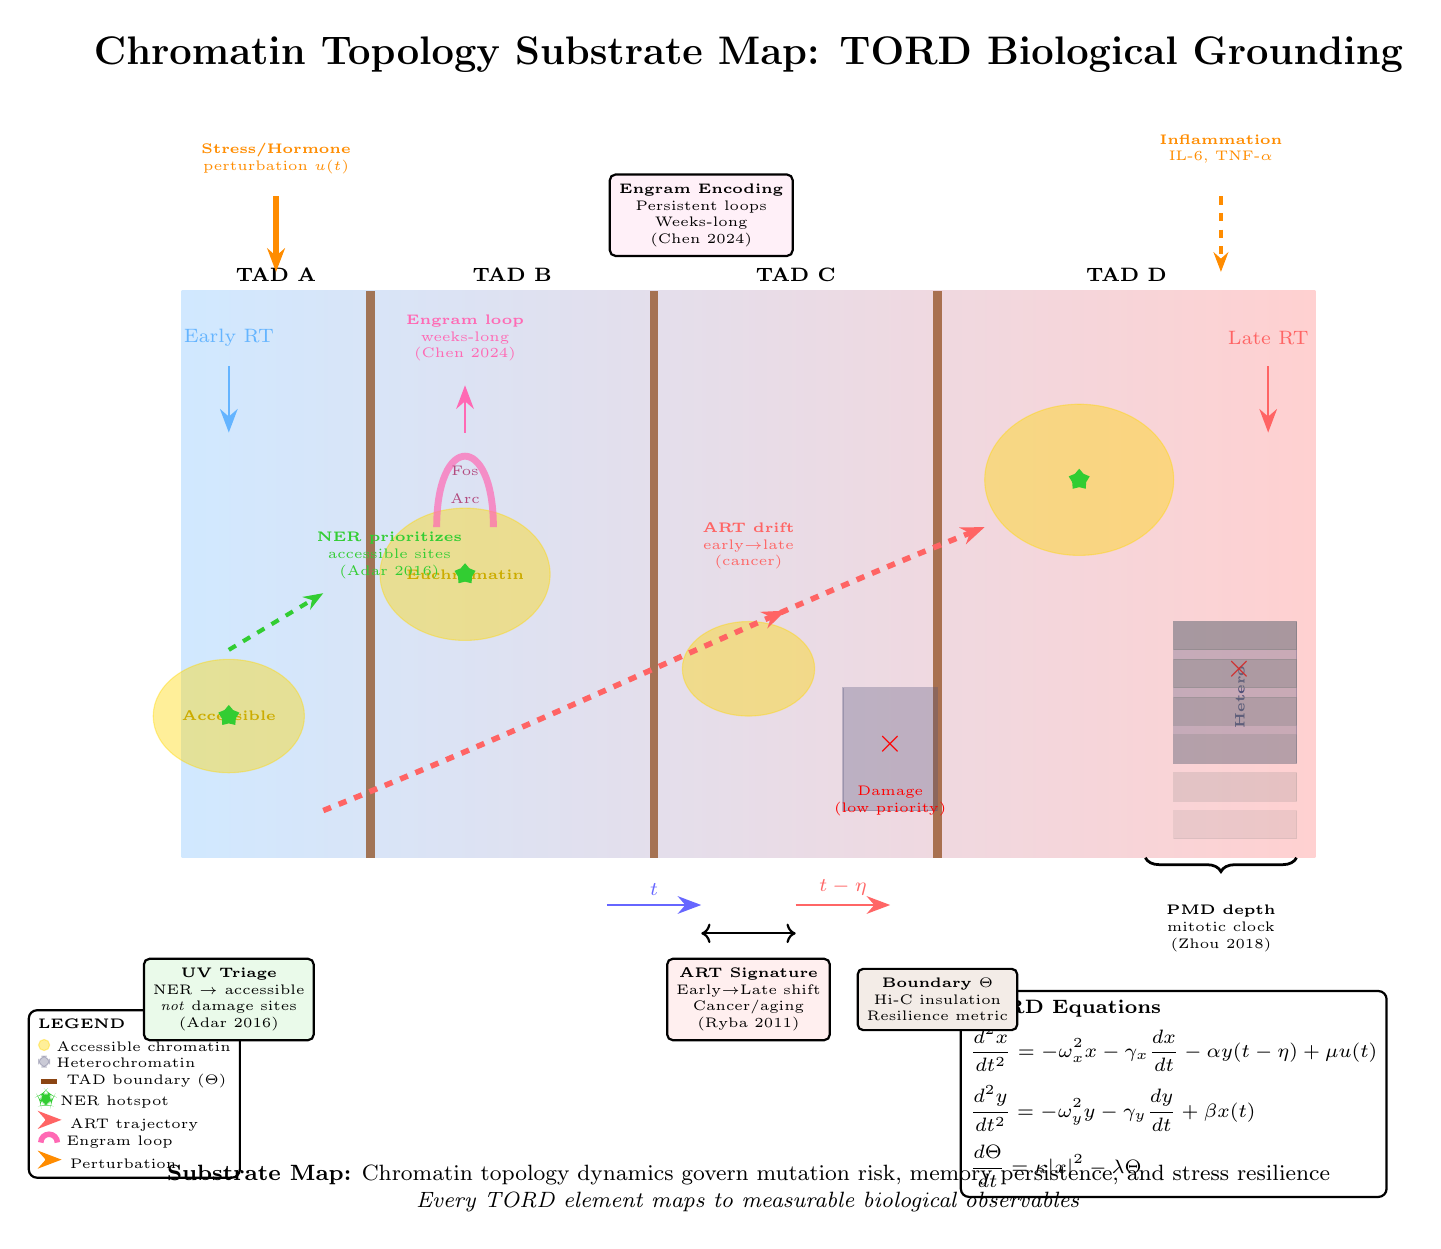
\begin{tikzpicture}[
    scale=1.2,
    every node/.style={font=\small},
    arrow/.style={-{Stealth[length=3mm]}, thick},
    dashedarrow/.style={-{Stealth[length=2.5mm]}, thick, dashed},
    region/.style={draw, thick, rounded corners=2pt},
    label/.style={font=\scriptsize\bfseries},
    ]

% ============================================================================
% TITLE
% ============================================================================
\node[font=\Large\bfseries] at (0, 8.5) {Chromatin Topology Substrate Map: TORD Biological Grounding};

% ============================================================================
% MAIN CHROMATIN LANDSCAPE
% ============================================================================

% Background gradient: Early to Late replication timing
\shade[left color=earlyRT!30, right color=lateRT!30]
    (-6, 0) rectangle (6, 6);

% TAD boundaries (vertical dividers)
\foreach \x in {-4, -1, 2} {
    \draw[boundary, line width=3pt, opacity=0.7] (\x, 0) -- (\x, 6);
}

% Label TADs
\node[label, above] at (-5, 6) {TAD A};
\node[label, above] at (-2.5, 6) {TAD B};
\node[label, above] at (0.5, 6) {TAD C};
\node[label, above] at (4, 6) {TAD D};

% Replication timing gradient annotation
\node[font=\scriptsize, text=earlyRT] at (-5.5, 5.5) {Early RT};
\draw[earlyRT, arrow] (-5.5, 5.2) -- (-5.5, 4.5);

\node[font=\scriptsize, text=lateRT] at (5.5, 5.5) {Late RT};
\draw[lateRT, arrow] (5.5, 5.2) -- (5.5, 4.5);

% ============================================================================
% ACCESSIBLE vs HETEROCHROMATIN REGIONS
% ============================================================================

% Accessible chromatin "bubbles" (euchromatin)
\filldraw[accessible, opacity=0.4] (-5.5, 1.5) ellipse (0.8 and 0.6);
\filldraw[accessible, opacity=0.4] (-3, 3) ellipse (0.9 and 0.7);
\filldraw[accessible, opacity=0.4] (0, 2) ellipse (0.7 and 0.5);
\filldraw[accessible, opacity=0.4] (3.5, 4) ellipse (1 and 0.8);

% Heterochromatin blocks
\filldraw[heterochromatin, opacity=0.3] (4.5, 1) rectangle (5.8, 2.5);
\filldraw[heterochromatin, opacity=0.3] (1, 0.5) rectangle (2, 1.8);

% Labels
\node[font=\tiny, text=accessible!80!black] at (-5.5, 1.5) {\textbf{Accessible}};
\node[font=\tiny, text=accessible!80!black] at (-3, 3) {\textbf{Euchromatin}};
\node[font=\tiny, text=heterochromatin] at (5.2, 1.7) {\rotatebox{90}{\textbf{Hetero}}};

% ============================================================================
% UV TRIAGE HOTSPOTS (NER priority)
% ============================================================================

% NER activity markers at ACCESSIBLE sites (not damage sites)
\node[star, star points=5, fill=NER, minimum size=8pt, inner sep=0] at (-5.5, 1.5) {};
\node[star, star points=5, fill=NER, minimum size=8pt, inner sep=0] at (-3, 3) {};
\node[star, star points=5, fill=NER, minimum size=8pt, inner sep=0] at (3.5, 4) {};

% UV damage symbols (not prioritized if in heterochromatin)
\node[font=\large, text=red] at (5.2, 2) {$\times$};
\node[font=\large, text=red] at (1.5, 1.2) {$\times$};
\node[font=\tiny, text=red, align=center] at (1.5, 0.6) {Damage\\(low priority)};

% NER annotation
\draw[NER, dashedarrow, line width=1.5pt] (-5.5, 2.2) -- (-4.5, 2.8);
\node[font=\tiny, text=NER, align=center] at (-3.8, 3.2) {\textbf{NER prioritizes}\\accessible sites\\(Adar 2016)};

% ============================================================================
% ART (Altered Replication Timing) TRAJECTORIES
% ============================================================================

% Trajectory showing early → late RT shift (cancer/aging)
\draw[lateRT, arrow, line width=2pt, dashed,
      decoration={markings, mark=at position 0.7 with {\arrow{Stealth[length=3mm]}}},
      postaction={decorate}]
    (-4.5, 0.5) .. controls (-2, 1.5) and (0, 2.5) .. (2.5, 3.5);

\node[font=\tiny, text=lateRT, align=center] at (0, 3.3) {\textbf{ART drift}\\early$\to$late\\(cancer)};

% ============================================================================
% PMD DEPTH ENCODING (mitotic clock)
% ============================================================================

% PMD region (partially methylated domain - aging signature)
\draw[decorate, decoration={brace, amplitude=5pt, mirror}, line width=1pt]
    (4.2, 0) -- (5.8, 0);
\node[font=\tiny, align=center, below] at (5, -0.4) {\textbf{PMD depth}\\mitotic clock\\(Zhou 2018)};

% Methylation gradient visualization
\foreach \y in {0.2, 0.6, 1.0, 1.4, 1.8, 2.2} {
    \filldraw[gray, opacity={0.1 + \y*0.15}] (4.5, \y) rectangle (5.8, \y+0.3);
}

% ============================================================================
% ENGRAM LOOPS (persistent chromatin loops)
% ============================================================================

% Persistent loop at learning locus
\draw[engram, line width=2.5pt, opacity=0.7]
    (-3.3, 3.5) .. controls (-3.3, 4.5) and (-2.7, 4.5) .. (-2.7, 3.5);
\draw[engram, arrow] (-3, 4.5) -- (-3, 5);
\node[font=\tiny, text=engram, align=center] at (-3, 5.5) {\textbf{Engram loop}\\weeks-long\\(Chen 2024)};

% Memory gene symbols inside loop
\node[font=\tiny, text=engram!70!black] at (-3, 3.8) {Arc};
\node[font=\tiny, text=engram!70!black] at (-3, 4.1) {Fos};

% ============================================================================
% STRESS PERTURBATION VECTORS
% ============================================================================

% Hormone/stress input arrows
\draw[stress, arrow, line width=2pt] (-5, 7) -- (-5, 6.2);
\node[font=\tiny, text=stress, align=center] at (-5, 7.4) {\textbf{Stress/Hormone}\\perturbation $u(t)$};

% Inflammation coupling
\draw[stress, dashedarrow, line width=1.5pt] (5, 7) -- (5, 6.2);
\node[font=\tiny, text=stress, align=center] at (5, 7.5) {\textbf{Inflammation}\\IL-6, TNF-$\alpha$};

% ============================================================================
% REPAIR DELAY PROPAGATION (η)
% ============================================================================

% Time delay visualization (repair lag)
\draw[thick, -{Stealth[length=3mm]}, color=blue!60]
    (-1.5, -0.5) -- (-0.5, -0.5);
\node[font=\scriptsize, color=blue!60, above] at (-1, -0.5) {$t$};

\draw[thick, -{Stealth[length=3mm]}, color=red!60]
    (0.5, -0.5) -- (1.5, -0.5);
\node[font=\scriptsize, color=red!60, above] at (1, -0.5) {$t - \eta$};

\draw[thick, <->, color=black] (-0.5, -0.8) -- (0.5, -0.8);
\node[font=\tiny, align=center, below] at (0, -1) {\textbf{Repair delay $\eta$}\\NER: 20min\\DSB: 2-4hr};

% ============================================================================
% LEGEND BOX
% ============================================================================

\node[draw, thick, rounded corners=3pt, fill=white, align=left, font=\tiny] at (-6.5, -2.5) {
\textbf{LEGEND}\\[2pt]
\tikz{\filldraw[accessible, opacity=0.4] (0,0) circle (2pt);} Accessible chromatin\\
\tikz{\filldraw[heterochromatin, opacity=0.3] (0,0) rectangle (4pt,4pt);} Heterochromatin\\
\tikz{\draw[boundary, line width=2pt] (0,0) -- (6pt,0);} TAD boundary ($\Theta$)\\
\tikz{\node[star, star points=5, fill=NER, minimum size=6pt, inner sep=0] at (0,0) {};} NER hotspot\\
\tikz{\draw[lateRT, arrow, dashed, line width=1.5pt] (0,0) -- (6pt,0);} ART trajectory\\
\tikz{\draw[engram, line width=2pt] (0,0) arc (180:0:3pt);} Engram loop\\
\tikz{\draw[stress, arrow, line width=1.5pt] (0,0) -- (6pt,0);} Perturbation
};

% ============================================================================
% TORD EQUATIONS (bottom right)
% ============================================================================

\node[draw, thick, rounded corners=3pt, fill=white, align=left, font=\scriptsize] at (4.5, -2.5) {
\textbf{TORD Equations}\\[2pt]
$\displaystyle \frac{d^2 x}{dt^2} = -\omega_x^2 x - \gamma_x \frac{dx}{dt} - \alpha y(t-\eta) + \mu u(t)$\\[4pt]
$\displaystyle \frac{d^2 y}{dt^2} = -\omega_y^2 y - \gamma_y \frac{dy}{dt} + \beta x(t)$\\[4pt]
$\displaystyle \frac{d\Theta}{dt} = \kappa |x|^2 - \lambda \Theta$
};

% ============================================================================
% KEY ANNOTATIONS
% ============================================================================

% Annotation 1: UV triage (top left)
\node[draw, thick, rounded corners=2pt, fill=NER!10, align=center, font=\tiny] at (-5.5, -1.5) {
\textbf{UV Triage}\\
NER $\to$ accessible\\
\textit{not} damage sites\\
(Adar 2016)
};

% Annotation 2: ART signature (middle)
\node[draw, thick, rounded corners=2pt, fill=lateRT!10, align=center, font=\tiny] at (0, -1.5) {
\textbf{ART Signature}\\
Early$\to$Late shift\\
Cancer/aging\\
(Ryba 2011)
};

% Annotation 3: Engram persistence (top)
\node[draw, thick, rounded corners=2pt, fill=engram!10, align=center, font=\tiny] at (-0.5, 6.8) {
\textbf{Engram Encoding}\\
Persistent loops\\
Weeks-long\\
(Chen 2024)
};

% Annotation 4: Boundary strength
\node[draw, thick, rounded corners=2pt, fill=boundary!10, align=center, font=\tiny] at (2, -1.5) {
\textbf{Boundary $\Theta$}\\
Hi-C insulation\\
Resilience metric
};

% ============================================================================
% BOTTOM TITLE
% ============================================================================

\node[font=\footnotesize, align=center] at (0, -3.5) {
\textbf{Substrate Map:} Chromatin topology dynamics govern mutation risk, memory persistence, and stress resilience\\
\textit{Every TORD element maps to measurable biological observables}
};

\end{tikzpicture}

\end{document}
